\documentclass[oneside, 11pt]{article}

\usepackage[T1]{fontenc}
\usepackage[utf8]{inputenc}
\usepackage[english]{babel}

\usepackage{fouriernc}
\usepackage[detect-all, binary-units, separate-uncertainty=true,
            per-mode=symbol, retain-explicit-plus, retain-unity-mantissa=false]{siunitx}

\usepackage{setspace}
\setstretch{1.2}

\setlength{\parskip}{\smallskipamount}
\setlength{\parindent}{0pt}

\usepackage[headheight=14pt]{geometry}
\geometry{marginparwidth=0.5cm, verbose, a4paper, tmargin=3cm, bmargin=3cm,
          lmargin=2cm, rmargin=2cm}

\usepackage{float}

\usepackage[fleqn]{amsmath}
\numberwithin{equation}{section}
\numberwithin{figure}{section}

\usepackage{graphicx}
\graphicspath{{images/}{../../../images/}}

\usepackage{tikz}
\usetikzlibrary{shapes}
\usetikzlibrary{plotmarks}

\newcounter{Exercise}
\setcounter{Exercise}{1}
\usepackage{xcolor}
\definecolor{shadecolor}{gray}{0.9}
\usepackage{framed}
\usepackage{caption}

\usepackage{url}


\usepackage{fancyhdr}
\pagestyle{fancy}
\fancyhf{}
\rhead{\thepage}
\renewcommand{\footrulewidth}{0pt}
\renewcommand{\headrulewidth}{0pt}

\fancypagestyle{firststyle}
{
    \fancyhf{}
    \rhead{\thepage}
    \cfoot{
\includegraphics[height=30pt]{HiSPARClogo}}
    \rfoot{
\includegraphics[height=25pt]{CCbysa}}
    \lfoot{
\includegraphics[height=30pt]{NIKHEFlogo}}
    \renewcommand{\footskip}{50pt}
    \renewcommand{\footrulewidth}{0.1pt}
    \renewcommand{\headrulewidth}{0pt}
}

\newcommand{\figref}[1]{Figuur~\ref{#1}}

\newcommand{\hisparc}{\textsmaller{HiSPARC}\xspace}
\newcommand{\kascade}{\textsmaller{KASCADE}\xspace}
\newcommand{\sapphire}{\textsmaller{SAPPHiRE}\xspace}
\newcommand{\jsparc}{\textsmaller{jSparc}\xspace}
\newcommand{\hdf}{\textsmaller{HDF5}\xspace}
\newcommand{\aires}{\textsmaller{AIRES}\xspace}
\newcommand{\csv}{\textsmaller{CSV}\xspace}
\newcommand{\python}{\textsmaller{PYTHON}\xspace}
\newcommand{\corsika}{\textsmaller{CORSIKA}\xspace}
\newcommand{\labview}{\textsmaller{LabVIEW}\xspace}
\newcommand{\daq}{\textsmaller{DAQ}\xspace}
\newcommand{\adc}{\textsmaller{ADC}\xspace}
\newcommand{\hi}{\textsc{h i}\xspace}
\newcommand{\hii}{\textsc{h ii}\xspace}
\newcommand{\mip}{\textsmaller{MIP}\xspace}
\newcommand{\hisparcii}{\textsmaller{HiSPARC II}\xspace}
\newcommand{\hisparciii}{\textsmaller{HiSPARC III}\xspace}

\DeclareSIUnit{\electronvolt}{\ensuremath{\mathrm{e\!\!\:V}}}

\DeclareSIUnit{\unitsigma}{\ensuremath{\sigma}}
\DeclareSIUnit{\mip}{\textsmaller{MIP}}
\DeclareSIUnit{\adc}{\textsmaller{ADC}}

\DeclareSIUnit{\gauss}{G}
\DeclareSIUnit{\parsec}{pc}
\DeclareSIUnit{\year}{yr}



\begin{document}

\title{Lenzen}
\author{N.G. Schultheiss}
\date{}

\maketitle
\thispagestyle{firststyle}

\section{Inleiding}

Deze module volgt op de module ``Spiegels''. Deze module wordt vervolgd
met de module ``Telescopen'' of de module ``Lenzen maken''. Uiteindelijk
kun je met de opgedane kennis een telescoop bouwen, de werking verklaren
of de telescoop als meetinstrument toepassen. Je hebt voor deze module
een passer, geodriehoek, potlood, papier en gum nodig.

Hieronder volgt een korte samenvatting van de kennis die je al beheerst.

Je kunt de lenzenwet $\frac{1}{f}=\frac{1}{b}+\frac{1}{v}$ toepassen
om een brandpuntafstand $f$, een voorwerpafstand $v$ of een beeldafstand
$b$ uit te rekenen als de andere twee grootheden gegeven zijn.

Je kunt de formule voor vergroting, $N=\frac{b}{v}=\frac{beeldgrootte}{voorwerpgrootte}$,
gebruiken om met drie gegeven grootheden de vierde grootheid uit te
rekenen. Je weet bijvoorbeeld $b$, $v$ en de $beeldgrootte$. Je
kunt de $voorwerpgrootte$ uitrekenen.

Je kunt het beeld van een voorwerp construeren met de drie bijzondere
constructiestralen.
\begin{itemize}
\item Een lichtstraal door het midden van een lens gaat rechtdoor.
\item Een lichtstraal die voor de lens evenwijdig aan de hoofdas gaat, gaat
na de lens door het brandpunt achter de lens.
\item Een lichtstraal die voor de lens door het brandpunt gaat, gaat na
de lens evenwijdig aan de hoofdas.
\end{itemize}
\begin{figure}[H]
\noindent \begin{centering}
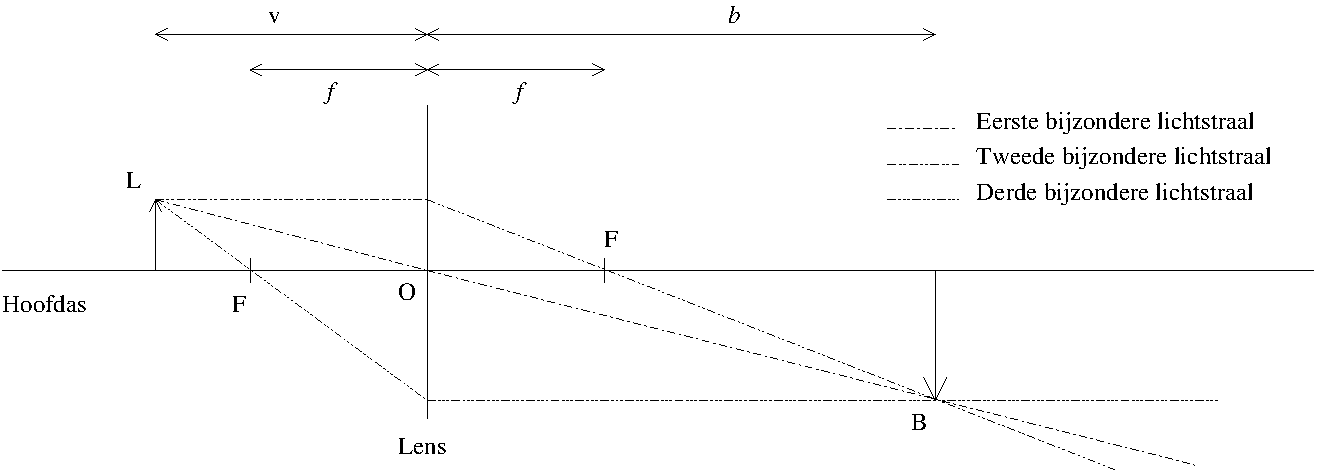
\includegraphics[scale=0.75]{constructie}
\par\end{centering}

\caption{De lensconstructie met drie bijzondere stralen}
\end{figure}


Zoals te zien is, worden de punten met een hoofdletter geschreven
en de afstanden met een kleine letter.\medskip{}


\qquad{}O: Optisch middelpunt (Het midden van de lens).

\qquad{}F: Focus of brandpunt.

\qquad{}L: Lichtpunt, het voorwerp straalt bij ieder lichtpunt licht
uit.

\qquad{}B: Beeldpunt.\newpage{}


\section{De werking van een lens}

Lenzen werken doordat licht en materie op elkaar inwerken. Als er geen
materie is, beweegt het licht met de lichtsnelheid \footnote{In 1676
stelde Ole R¯mer de lichtsnelheid vast op 225 000 km/s. Hij vond deze
snelheid door de tijden te vergelijken, waarop de maan Io van Jupiter
achter Jupiter (eclips) tevoorschijn komt (dit is beschreven op
wikipedia). } $c$. Tegenwoordig definieert men de eenheid {[}m{]} uit de
lichtsnelheid in vacuum en geldt $c=299792458\mathrm{[m/s]}$ exact.

Het zal duidelijk zijn dat licht alleen door doorzichtige materie
gaat. De lichtsnelheid neemt dan echter altijd af. Het licht gaat
in water ongeveer met $\frac{3}{4}$ van de lichtsnelheid, in glas
is de snelheid ongeveer $\frac{2}{3}$ van de lichtsnelheid. Omdat
het licht een kleinere snelheid krijgt, zal de lichtstraal breken.


\paragraph*{Opdracht 1:}

\emph{In de module ``Spiegels'' hebben we kennisgemaakt met het
Huygens-principe. Leg uit wat er gebeurt als we de afstand tussen
de golffronten in luchtledig (zonder materie) en water vergelijken.}

\begin{figure}[H]
\noindent \begin{centering}
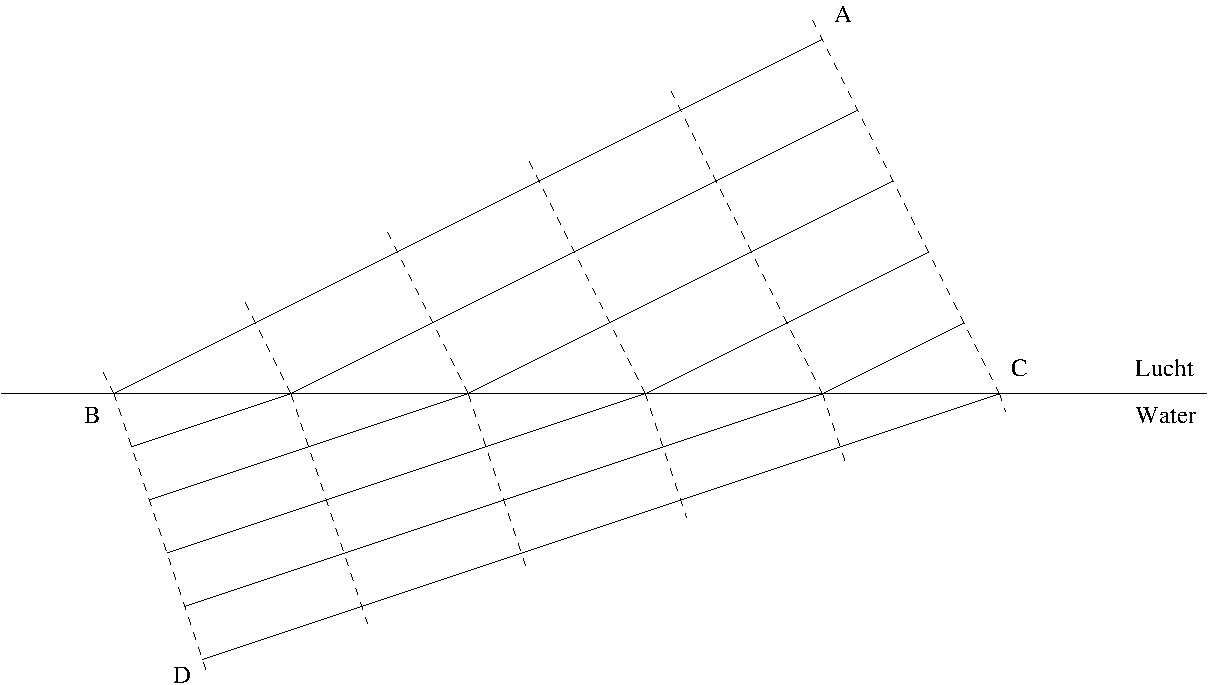
\includegraphics[scale=0.75]{breking}
\par\end{centering}

\caption{Breking aan een lucht / water oppervlak}
\end{figure}


In figuur 2.1 zijn twee driehoeken te zien: $\triangle\mathrm{ABC}$
en $\triangle\mathrm{BCD}$. Het is direct duidelijk dat het lijnstuk
$(\mathrm{BC})$ in beide driehoeken zit. We weten al dat het golffront
loodrecht op de golfstraal staat: $\angle\mathrm{BAC}=\angle\mathrm{BDC}=90^{o}$.


\paragraph*{Opdracht 2:}

\emph{Leg uit hoe je de waarde van $\sin(\angle\mathrm{ABC})$ kunt
bepalen.}


\paragraph*{Opdracht 3:}

\emph{Leg uit hoe je de waarde van $\sin(\angle\mathrm{BCD})$ kunt
bepalen.}


\paragraph*{Opdracht 4:}

\emph{Toon aan dat de onderstaande formule geldt:}

\[
\frac{\sin(\angle\mathrm{ABC})}{\sin(\angle\mathrm{BCD})}
=\frac{(\mathrm{AC})}{(\mathrm{BD})}
\]



\paragraph*{Opdracht 5:}

\emph{Leg uit dat de verhouding $\frac{(\mathrm{AC})}{(\mathrm{BD})}$
gelijk is aan de verhouding van de lichtsnelheden.}

De verhouding van de lichtsnelheden wordt in dit geval de brekingsindex
$N_{lucht\rightarrow water}$ genoemd.


\paragraph*{Opdracht 6:}

\emph{Toon aan dat de hoeken $\angle\mathrm{ABC}$ en $\angle\mathrm{BCD}$
gelijk zijn aan de hoek van inval $i$ (tussen de invallende straal
en de normaal) en de hoek van breking $r$ (tussen de gebroken straal
en de normaal).}


\paragraph*{Opdracht 7:}

Verklaar de onderstaande formule \footnote{Deze formule is in Nederland
bekend onder de naam: ``De wet van Snellius''. Hij is vernoemd naar
Willibrord Snell van Royen, die een dergelijk relatie voor het eerst
wiskundig opschreef. Deze schrijfwijze is echter door René Descartes
geformuleerd, in Frankrijk is dit dus de wet van Descartes.}:

\[
N=\frac{\sin(i)}{\sin(r)}
\]



\section{De constructie voor breking aan vlakke en bolvormige oppervlakken}

Het tekenen van alle golffronten en golfstralen is een omslachtige
klus. We gebruiken daarom twee constructies waarmee we de breking
aan vlakke en bolvormige oppervlakken kunnen bepalen. We kunnen de
lichtstraal (ray) daarmee volgen, deze techniek heet raytracing.

\begin{figure}[H]
\noindent \begin{centering}
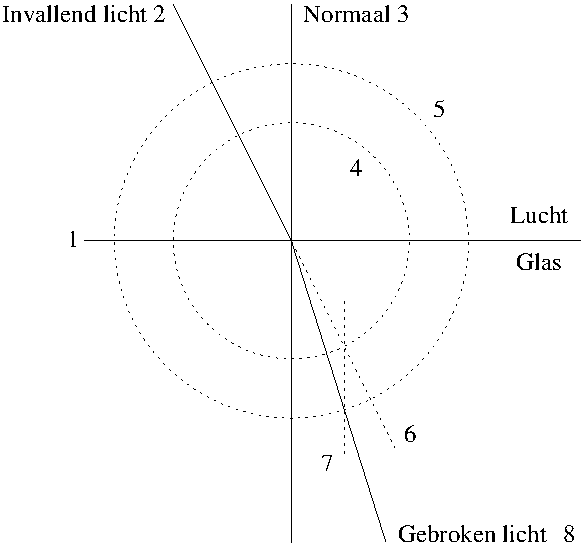
\includegraphics[scale=0.75]{vlak}
\par\end{centering}

\caption{De breking aan een plat vlak}
\end{figure}


In figuur 3.1 zijn diverse getallen gegeven. Deze geven aan welke
procedure gevolgd wordt:
\begin{enumerate}
\item Teken het oppervlak tussen beide materialen, hier lucht en glas.
\item Teken de invallende lichtstraal.
\item Teken de normaal bij het snijpunt van de invallende lichtstraal en
het oppervlak. Uiteraard staat de normaal loodrecht op het oppervlak.
\item Teken een cirkel met als middelpunt het snijpunt, hier geldt bijvoorbeeld
$r=1.5[\mathrm{cm}]$.
\item Teken een tweede concentrische cirkel waarvan de straal $N$ maal
groter is dan de straal van de eerste cirkel, hier geldt bijvoorbeeld
$r=2.25[\mathrm{cm}]$. 
\item Trek de invallende lichtstraal (gestippeld) door. 
\item Trek een lijn (gestippeld) evenwijdig aan de hoofdas door de cirkel
(4) en de lijn (6).
\item Trek de gebroken lichtstraal van het midden door het snijpunt van
de cirkel (5) en de lijn (7).
\end{enumerate}

\paragraph*{Opdracht 8:}

\emph{Een lichtstraal valt met een hoek $i=25^{o}$op een diamant
met $N_{lucht\rightarrow diamant}=2,417$. Construeer de gebroken
lichtstraal.\newpage{}}

Bij de constructie aan een bolvormig oppervlak hebben we drie cirkels
nodig.

\begin{figure}[H]
\noindent \begin{centering}
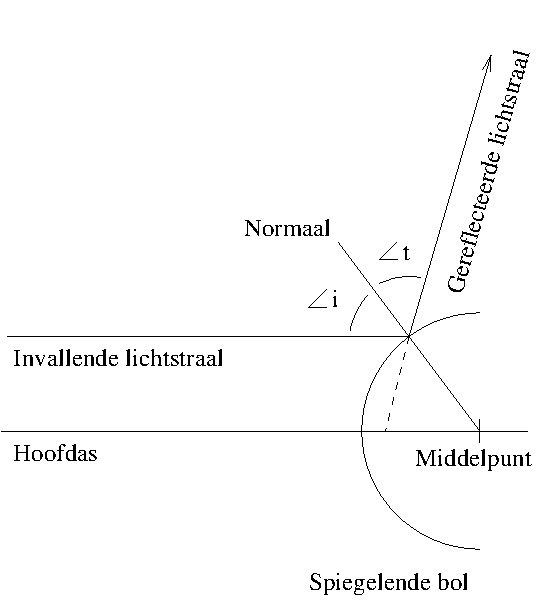
\includegraphics[scale=0.75]{bol}
\par\end{centering}

\caption{De breking aan een bol oppervlak}
\end{figure}


In figuur 3.2 zijn diverse getallen gegeven. Deze geven aan welke
procedure gevolgd wordt:
\begin{enumerate}
\item Teken de hoofdas.
\item Teken het bolvormig oppervlak. Let op dat je het middelpunt van de
cirkel vastlegt. (Hier geldt $r=3,6[\mathrm{cm}]$).
\item Teken de invallende lichtstraal.
\item Teken een hulpcirkel. De straal hiervan is de brekingsindex keer zo
groot als de straal van het oppervlak. (Hier geldt $r=4,8[\mathrm{cm}]$).
\item Teken een hulpcirkel. De straal hiervan is de brekingsindex keer zo
klein als de straal van het oppervlak. (Hier geldt $r=2,7[\mathrm{cm}]$).
\item Trek de invallende lichtstraal door naar de buitenste cirkel (4).
\item Trek een lijn van dit snijpunt naar het midden van de cirkel.
\item Trek de gebroken straal door het snijpunt van de cirkel (5) en de
lijn (7).
\end{enumerate}
Soms hoeven we niet precies te weten hoe de lichtstraal loopt maar
willen we wel voorspellen welke brandpuntsafstand een lens heeft.
Dit kan met de lenzenmakersformule:

\[
\frac{1}{f}=(N-1)(\frac{1}{r_{1}}-\frac{1}{r_{2}})
\]


Let op, de afspraak is dat alle afstanden naar rechts positief zijn
en naar links negatief zijn. Bij een lens met twee bollekanten (biconvex)
is de straal $r_{1}$ (van oppervlak naar middelpunt) positief en
de straal $r_{2}$ (ook van oppervlak naar middelpunt) negatief.\newpage{}

Als we de maten en de brekingsindex van een lens kennen, kunnen we
de brandpuntsafstand uitrekenen. Een lens met $r_{1}=10,0[\mathrm{cm}]$,
$r_{2}=5,0[\mathrm{cm}]$ en $N_{lens}=1,50$ geeft de volgende brandpuntsafstand:

\[
\frac{1}{f}=(1,50-1)(\frac{1}{0,10}-\frac{1}{-0,050})
\]


\[
\frac{1}{f}=(0,50)(10+20)
\]


\[
\frac{1}{f}=15
\]


\[
f=\frac{1}{15}[\mathrm{m}]=6,7\mathrm{[cm]}
\]


\begin{figure}[H]
\noindent \begin{centering}
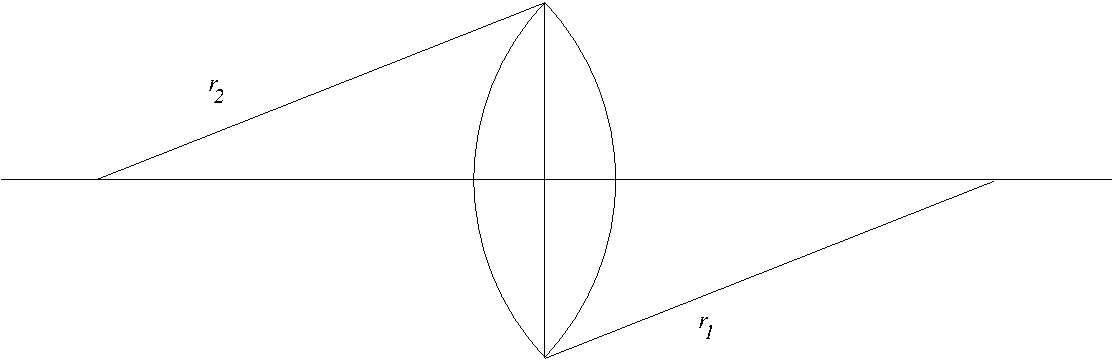
\includegraphics[scale=0.75]{lens}
\par\end{centering}

\caption{Een lens}
\end{figure}



\paragraph*{Opdracht 9:}

\emph{Bereken de brandpuntsafstand van een planconvex lens met $r_{1}=\infty$
en $r_{2}=4,0[\mathrm{cm}]$. De voorkant is dus plat en de achterkant
is bol. De brekingsindex $N=2,0$.}


\paragraph*{Opdracht 10:}

\emph{Controleer je berekening met een constructie voor twee evenwijdig
aan de hoofdas lopende invallende stralen. Neem deze op }1,0{[}cm{]}\emph{
en }2,0{[}cm{]}\emph{ van de hoofdas.}


\paragraph*{Opdracht 11:}

\emph{Krijg je met de constructie een goed brandpunt, wat is de brandpuntsafstand?}

Als je nauwkeurig met een scherp potlood hebt gewerkt, krijg je toch
geen scherp brandpunt. Deze lensfout noemt men sferische abberatie.

\end{document}
